\section{Durchführung}
\label{sec:Durchführung}
Die Durchführung dieses Versuches erfolgt mit einem D8-Diffraktometer der Firma Bruker-AXS.
Zur Erzeugung der Röntgenstrahlung ist in diesem eine Röntgenröhre mit Kupferanode verbaut, welche mit einem Strom von $\SI{35}{\mA}$ und einer Spannung von $\SI{40}{\kV}$ betrieben wird.
Der austretende Strahl besitzt einer Wellenlänge von $\lambda = \SI{1,54}{\angstrom}$ und eine Intensität von $10^7 - 10^8$ Photonen pro Sekunde auf einer Fläche von $\SI{0,1}{\mm}\times\SI{1}{\cm}$.
Durch Reflexion an einem Göbel-Spiegel wird die divergente Strahlung parallelisiert.
Anschließend durchläuft der Strahl einen Autoabsorber und eine Blende, sodass er mit reduzierter Intensität auf die Probe trifft.
Nach der Reflexion an der Probe wird unerwünschte Streustrahlung durch einen Spalt ausgeblendet und nachdem der Strahl eine weitere Blende passiert hat, trifft er auf den Detektor.
Der schematische Verlauf der Strahlung ist in Abbildung \ref{fig:tfig6} dargestellt.
\begin{figure}[H]
\centering
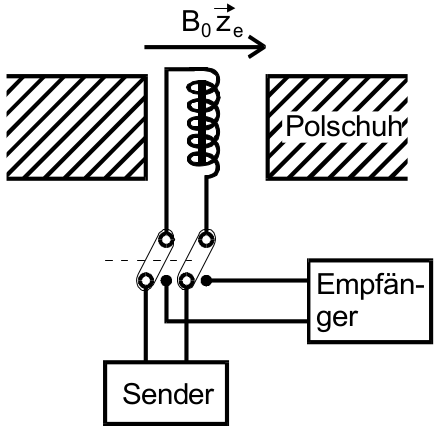
\includegraphics[width=0.7\linewidth]{figures/Aufbau}
\caption{Schematische Darstellung des Verlaufs der Röntgenstrahlung zwischen Röntgenröhre, Probe und Detektor \cite{skript}}
\label{fig:tfig6}
\end{figure}

Vor Beginn der Messung erfolgt die Justierung, für welche die drei Messmethoden \textit{Detektorscan}, \textit{Z-Scan} und \textit{Rocking-Scan} zur Verfügung stehen.
Die verwendeten Parameter jeder Messung sind in Tabelle \ref{tab:ttab1} aufgeführt.
Zunächst wird ein Detektorscan zur Justierung des Primärstrahls durchgeführt, welcher den Detektor in einem kleinen Winkelbereich um die Probe der Röhre bewegt.
Aus diesem Scan ergibt sich eine Gaußglocke auf dessen Maximum die Nulllage des Detektor kalibriert wird.
Anschließend wird die Probe auf den Probentisch nach Augenmaß positioniert, indem die $x$-$y$- und $z$-Koordinaten des Tisches entsprechend verändert werden.

Die Probe soll so positioniert werden, dass sie parallel zum Strahl steht und die halbe Intensität des Primärstrahls abschirmt.
Hierzu wird nacheinander die z-Koordinate und die Verkippung der Probe justiert.
Der Z-Scan dient zur Optimierung der z-Koordinate der Probe.
Hierbei wird die Probe in z-Richtung verschoben, die Intensität gemessen und anschließend die z-Koordinate der Probe an die Stelle gesetzt an welcher die Intensität halbiert ist.
Der Rocking-Scan dient dazu die Verkippung der Probe im Strahl zu kalibrieren.
Bei diesem drehen sich Röhre und Detektor um die Probe, wobei der Winkel zwischen Detektor und Röhre konstant bleibt.
Die sich hieraus ergebene Intensitätsverteilung soll einem symmetrischen Dreieck entsprechen.
Ist dieses nicht der Fall wird die Position des Probentisches angepasst.
Sobald das Dreieck symmetrisch ist, wird die Position des Maximums an die Motoren übermittelt.
Anschließend wird ein erneuter Z-Scan durchgeführt.
Zuletzt wird ein weitere Rocking-Scan und ein dritter Z-Scan diesmal aber unter einem Winkel von $0,15°$ durchgeführt.
\begin{table}[H]
    \centering
    \caption{Werte für die Justierung der Apparatur. Die Messdauer pro Messpunkt beträgt jeweils $\SI{1}{\s}$.}
    \label{tab:ttab1}
    \begin{tabular}{l c c }
        \toprule
        {Typ} & {Messbereich} & {Schrittweite}\\
        \midrule
        Detektorscan                    & -0,5 bis 0,5   & 0,02 \\
        Z-Scan                          & -1 bis 1       & 0,04 \\
        Rocking-Scan                    & -1 bis 1       & 0,04 \\
        Z-Scan                          & -0,5 bis 0,5   & 0,02 \\
        Rocking-Scan $2\theta = 0,3°$   & 0 bis 0,3      & 0,005\\
        Z-Scan $2\theta = 0,3°$         & -0,5 bis 0,5   & 0,02 \\
        \bottomrule
    \end{tabular}
\end{table}

Die Messung eines Polymerfilms auf einem Siliziumpaper erfolgt mittels eines \textit{Reflektivitätsscans}.
Bei diesem ist der Einfallswinkel $\alpha_1$ auf die Probe gleich dem Winkel $\alpha_f$ zwischen Probe und Detektor.
Die Messung erfolgt in einem Scanbereich von $0°$ bis $2,5°$, mit einer Schrittweite von $0,005°$ und einer Messzeit von $\SI{5}{\s}$ pro Messpunkt.
Um den Anteil der gestreuten Reflektivität an der Reflektivität zu bestimmen wird zuletzt noch ein \textit{Diffuser Scan} durchgeführt.
Dieser erfolgt unter den selben Einstellungen wie der vorherige Scan nur dass der Detektorwinkel um $0,1°$ gegenüber dem Einfallswinkel verschoben wird.
